\section{GtkSignalListItemFactory}\label{gtksignallistitemfactory}

\subsection{GtkSignalListItemFactory and
GtkBulderListItemFactory}\label{gtksignallistitemfactory-and-gtkbulderlistitemfactory}

GtkBuilderlistItemFactory is convenient when GtkListView just shows the
contents of a list. Its binding direction is always from an item of a
list to a child of GtkListItem.

When it comes to dynamic connection, it's not enough. For example,
suppose you want to edit the contents of a list. You set a child of
GtkListItem to a GtkText instance so a user can edit a text with it. You
need to bind an item in the list with the buffer of the GtkText. The
direction is opposite from the one with GtkBuilderListItemFactory. It is
from the GtkText instance to the item in the list. You can implement
this with GtkSignalListItemFactory, which is more flexible than
GtkBuilderListItemFactory.

This section shows just some parts of the source file
\passthrough{\lstinline!listeditor.c!}. If you want to see the whole
codes, see \passthrough{\lstinline!src/listeditor!} directory of the
\href{https://github.com/ToshioCP/Gtk4-tutorial}{Gtk4 tutorial
repository}.

\subsection{A list editor}\label{a-list-editor}

The sample program is a list editor and data of the list are strings.
It's the same as a line editor. It reads a text file line by line. Each
line is an item of the list. The list is displayed with GtkColumnView.
There are two columns. The one is a button, which shows if the line is a
current line. If the line is the current line, the button is colored
with red. The other is a string which is the contents of the
corresponding item of the list.

\begin{figure}
\centering
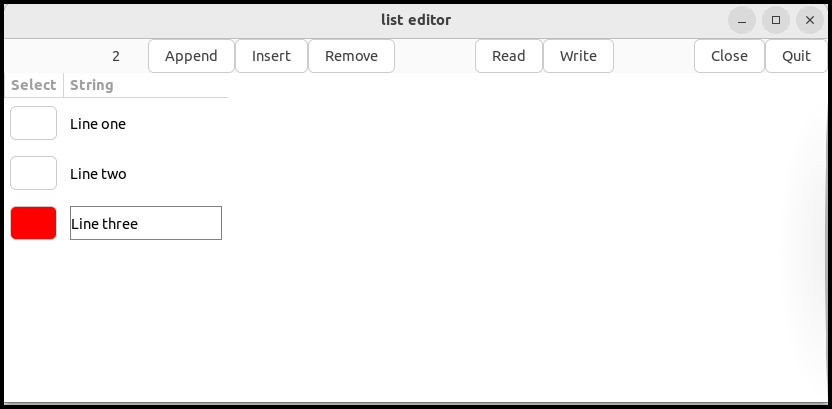
\includegraphics[width=12cm,height=9cm]{../image/listeditor.png}
\caption{List editor}
\end{figure}

The source files are located at \passthrough{\lstinline!src/listeditor!}
directory. You can compile end execute it as follows.

\begin{itemize}
\tightlist
\item
  Download the program from the
  \href{https://github.com/ToshioCP/Gtk4-tutorial}{repository}.
\item
  Change your current directory to
  \passthrough{\lstinline!src/listeditor!}.
\item
  Type the following on your commandline.
\end{itemize}

\begin{lstlisting}
$ meson setup _build
$ ninja -C _build
$ _build/listeditor
\end{lstlisting}

\begin{itemize}
\tightlist
\item
  Append button: appends a line after the current line, or at the last
  line if no current line exists.
\item
  Insert button: inserts a line before the current line, or at the top
  line if no current line exists.
\item
  Remove button: removes a current line.
\item
  Read button: reads a file.
\item
  Write button: writes the contents to a file.
\item
  close button: closes the contents.
\item
  quit button: quits the application.
\item
  Button on the select column: makes the line current.
\item
  String column: GtkText. You can edit a string in the field.
\end{itemize}

The current line number (zero-based) is shown at the left of the tool
bar. The file name is shown at the right of the write button.

\subsection{Connect a GtkText instance and an item in the
list}\label{connect-a-gtktext-instance-and-an-item-in-the-list}

The second column (GtkColumnViewColumn) sets its factory property to
GtkSignalListItemFactory. It uses three signals setup, bind and unbind.
The following shows the signal handlers.

\begin{lstlisting}[language=C, numbers=left]
static void
setup2_cb (GtkListItemFactory *factory, GtkListItem *listitem) {
  GtkWidget *text = gtk_text_new ();
  gtk_list_item_set_child (listitem, GTK_WIDGET (text));
  gtk_editable_set_alignment (GTK_EDITABLE (text), 0.0);
}

static void
bind2_cb (GtkListItemFactory *factory, GtkListItem *listitem) {
  GtkWidget *text = gtk_list_item_get_child (listitem);
  GtkEntryBuffer *buffer = gtk_text_get_buffer (GTK_TEXT (text));
  LeData *data = LE_DATA (gtk_list_item_get_item(listitem));
  GBinding *bind;

  gtk_editable_set_text (GTK_EDITABLE (text), le_data_look_string (data));
  gtk_editable_set_position (GTK_EDITABLE (text), 0);

  bind = g_object_bind_property (buffer, "text", data, "string", G_BINDING_DEFAULT);
  g_object_set_data (G_OBJECT (listitem), "bind", bind);
}

static void
unbind2_cb (GtkListItemFactory *factory, GtkListItem *listitem) {
  GBinding *bind = G_BINDING (g_object_get_data (G_OBJECT (listitem), "bind"));

  if (bind)
    g_binding_unbind(bind);
  g_object_set_data (G_OBJECT (listitem), "bind", NULL);
}
\end{lstlisting}

\begin{itemize}
\tightlist
\item
  1-6: \passthrough{\lstinline!setup2\_cb!} is a setup signal handler on
  the GtkSignalListItemFactory. This factory is inserted to the factory
  property of the second GtkColumnViewColumn. The handler just creates a
  GtkText instance and sets the child of
  \passthrough{\lstinline!listitem!} to it. The instance will be
  destroyed automatically when the \passthrough{\lstinline!listitem!} is
  destroyed. So, teardown signal handler isn't necessary.
\item
  8-20: \passthrough{\lstinline!bind2\_cb!} is a bind signal handler. It
  is called when the \passthrough{\lstinline!listitem!} is bound to an
  item in the list. The list items are LeData instances. LeData is
  defined in the file \passthrough{\lstinline!listeditor.c!} (the C
  source file of the list editor). It is a child class of GObject and
  has string data which is the content of the line.

  \begin{itemize}
  \tightlist
  \item
    10-11: \passthrough{\lstinline!text!} is a child of the
    \passthrough{\lstinline!listitem!} and it is a GtkText instance. And
    \passthrough{\lstinline!buffer!} is a GtkEntryBuffer instance of the
    \passthrough{\lstinline!text!}.
  \item
    12: The LeData instance \passthrough{\lstinline!data!} is an item
    pointed by the \passthrough{\lstinline!listitem!}.
  \item
    15-16: Sets the text of \passthrough{\lstinline!text!} to
    \passthrough{\lstinline!le\_data\_look\_string (data)!}.
    le\_data\_look\_string returns the string of the
    \passthrough{\lstinline!data!} and the ownership of the string is
    still taken by the \passthrough{\lstinline!data!}. So, the caller
    doesn't need to free the string.
  \item
    18: \passthrough{\lstinline!g\_object\_bind\_property!} binds a
    property and another object property. This line binds the ``text''
    property of the \passthrough{\lstinline!buffer!} (source) and the
    ``string'' property of the \passthrough{\lstinline!data!}
    (destination). It is a uni-directional binding
    (\passthrough{\lstinline!G\_BINDING\_DEFAULT!}). When a user changes
    the GtkText text, the same string is immediately put into the
    \passthrough{\lstinline!data!}. The function returns a GBinding
    instance. This binding is different from bindings of GtkExpression.
    This binding needs the existence of the two properties.
  \item
    19: GObjec has a table. The key is a string (or GQuark) and the
    value is a gpointer (pointer to any type). The function
    \passthrough{\lstinline!g\_object\_set\_data!} sets the association
    from the key to the value. This line sets the association from
    ``bind'' to \passthrough{\lstinline!bind!} instance. It makes
    possible for the ``unbind'' handler to get the
    \passthrough{\lstinline!bind!} instance.
  \end{itemize}
\item
  22-29: \passthrough{\lstinline!unbind2\_cb!} is a unbind signal
  handler.

  \begin{itemize}
  \tightlist
  \item
    24: Retrieves the \passthrough{\lstinline!bind!} instance from the
    table in the \passthrough{\lstinline!listitem!} instance.
  \item
    26-27: Unbind the binding.
  \item
    28: Removes the value corresponds to the ``bind'' key.
  \end{itemize}
\end{itemize}

This technique is not so complicated. You can use it when you make a
cell editable application.

If it is impossible to use
\passthrough{\lstinline!g\_object\_bind\_property!}, use a notify signal
on the GtkEntryBuffer instance. You can use ``deleted-text'' and
``inserted-text'' signal instead. The handler of the signals above
copies the text in the GtkEntryBuffer instance to the LeData string.
Connect the notify signal handler in \passthrough{\lstinline!bind2\_cb!}
and disconnect it in \passthrough{\lstinline!unbind2\_cb!}.

\subsection{Change the cell of GtkColumnView
dynamically}\label{change-the-cell-of-gtkcolumnview-dynamically}

Next topic is to change the GtkColumnView (or GtkListView) cells
dynamically. The example changes the color of the buttons, which are
children of GtkListItem instances, as the current line position moves.

The line editor has the current position of the list.

\begin{itemize}
\tightlist
\item
  At first, no line is current.
\item
  When a line is appended or inserted, the line is current.
\item
  When the current line is deleted, no line will be current.
\item
  When a button in the first column of GtkColumnView is clicked, the
  line will be current.
\item
  It is necessary to set the line status (whether current or not) when a
  GtkListItem is bound to an item in the list. It is because GtkListItem
  is recycled. A GtkListItem was possibly current line before but not
  current after recycled. The opposite can also be happen.
\end{itemize}

The button of the current line is colored with red and otherwise white.

The current line has no relationship to GtkSingleSelection object.
GtkSingleSelection selects a line on the display. The current line
doesn't need to be on the display. It is possible to be on the line out
of the Window (GtkScrolledWindow). Actually, the program doesn't use
GtkSingleSelection.

The LeWindow instance has two instance variables for recording the
current line.

\begin{itemize}
\tightlist
\item
  \passthrough{\lstinline!win->position!}: An int type variable. It is
  the position of the current line. It is zero-based. If no current line
  exists, it is -1.
\item
  \passthrough{\lstinline!win->current\_button!}: A variable points the
  button, located at the first column, on the current line. If no
  current line exists, it is NULL.
\end{itemize}

If the current line moves, the following two functions are called. They
updates the two varables.

\begin{lstlisting}[language=C, numbers=left]
static void
update_current_position (LeWindow *win, int new) {
  char *s;

  win->position = new;
  if (win->position >= 0)
    s = g_strdup_printf ("%d", win->position);
  else
    s = "";
  gtk_label_set_text (GTK_LABEL (win->position_label), s);
  if (*s) // s isn't an empty string
    g_free (s);
}

static void
update_current_button (LeWindow *win, GtkButton *new_button) {
  const char *non_current[1] = {NULL};
  const char *current[2] = {"current", NULL};

  if (win->current_button) {
    gtk_widget_set_css_classes (GTK_WIDGET (win->current_button), non_current);
    g_object_unref (win->current_button);
  }
  win->current_button = new_button;
  if (win->current_button) {
    g_object_ref (win->current_button);
    gtk_widget_set_css_classes (GTK_WIDGET (win->current_button), current);
  }
}
\end{lstlisting}

The varable \passthrough{\lstinline!win->position\_label!} points a
GtkLabel instance. The label shows the current line position.

The current button has CSS ``current'' class. The button is colored red
through the CSS ``button.current \{background: red;\}''.

The order of the call for these two functions is important. The first
function, which updates the position, is usually called first. After
that, a new line is appended or inserted. Then, the second function is
called.

The following functions call the two functions above. Be careful about
the order of the call.

\begin{lstlisting}[language=C, numbers=left]
void
select_cb (GtkButton *btn, GtkListItem *listitem) {
  LeWindow *win = LE_WINDOW (gtk_widget_get_ancestor (GTK_WIDGET (btn), LE_TYPE_WINDOW));

  update_current_position (win, gtk_list_item_get_position (listitem));
  update_current_button (win, btn);
}

static void
setup1_cb (GtkListItemFactory *factory, GtkListItem *listitem) {
  GtkWidget *button = gtk_button_new ();
  gtk_list_item_set_child (listitem, button);
  gtk_widget_set_focusable (GTK_WIDGET (button), FALSE);
  g_signal_connect (button, "clicked", G_CALLBACK (select_cb), listitem);
}

static void
bind1_cb (GtkListItemFactory *factory, GtkListItem *listitem, gpointer user_data) {
  LeWindow *win = LE_WINDOW (user_data);
  GtkWidget *button = gtk_list_item_get_child (listitem);

  if (win->position == gtk_list_item_get_position (listitem))
    update_current_button (win, GTK_BUTTON (button));
}
\end{lstlisting}

\begin{itemize}
\tightlist
\item
  1-7: \passthrough{\lstinline!select\_cb!} is a ``clicked'' signal
  handler. The handler just calls the two functions and update the
  position and button.
\item
  9-15: \passthrough{\lstinline!setup1\_cb!} is a setup signal handler
  on the GtkSignalListItemFactory. It sets the child of
  \passthrough{\lstinline!listitem!} to a GtkButton instance. The
  ``clicked'' signal on the button is connected to the handler
  \passthrough{\lstinline!select\_cb!}. When the listitem is destroyed,
  the child (GtkButton) is also destroyed. At the same time, the
  connection of the signal and the handler is also destroyed. So, you
  don't need teardown signal handler.
\item
  17-24: \passthrough{\lstinline!bind1\_cb!} is a bind signal handler.
  Usually, the position moves before this handler is called. If the item
  is on the current line, the button is updated. No unbind handler is
  necessary.
\end{itemize}

When a line is added, the current position is updated in advance.

\begin{lstlisting}[language=C, numbers=left]
static void
app_cb (GtkButton *btn, LeWindow *win) {
  LeData *data = le_data_new_with_data ("");

  if (win->position >= 0) {
    update_current_position (win, win->position + 1);
    g_list_store_insert (win->liststore, win->position, data);
  } else {
    update_current_position (win, g_list_model_get_n_items (G_LIST_MODEL (win->liststore)));
    g_list_store_append (win->liststore, data);
  }
  g_object_unref (data);
}

static void
ins_cb (GtkButton *btn, LeWindow *win) {
  LeData *data = le_data_new_with_data ("");

  if (win->position >= 0)
    g_list_store_insert (win->liststore, win->position, data);
  else {
    update_current_position (win, 0);
    g_list_store_insert (win->liststore, 0, data);
  }
  g_object_unref (data);
}
\end{lstlisting}

When a line is removed, the current position becomes -1 and no button is
current.

\begin{lstlisting}[language=C, numbers=left]
static void
rm_cb (GtkButton *btn, LeWindow *win) {
  if (win->position >= 0) {
    g_list_store_remove (win->liststore, win->position);
    update_current_position (win, -1);
    update_current_button (win, NULL);
  }
}
\end{lstlisting}

The color of buttons are determined by the ``background'' CSS style. The
following CSS node is a bit complicated. CSS node
\passthrough{\lstinline!column view!} has
\passthrough{\lstinline!listview!} child node. It covers the rows in the
GtkColumnView. The \passthrough{\lstinline!listview!} node is the same
as the one for GtkListView. It has \passthrough{\lstinline!row!} child
node, which is for each child widget. Therefore, the following node
corresponds buttons on the GtkColumnView widget. In addition, it is
applied to the ``current'' class.

\begin{lstlisting}
columnview listview row button.current {background: red;}
\end{lstlisting}

\subsection{A waring from GtkText}\label{a-waring-from-gtktext}

If your program has the following two, a warning message can be issued.

\begin{itemize}
\tightlist
\item
  The list has many items and it needs to be scrolled.
\item
  A GtkText instance is the focus widget.
\end{itemize}

\begin{lstlisting}
GtkText - unexpected blinking selection. Removing
\end{lstlisting}

I don't have an exact idea why this happens. But if GtkText
``focusable'' property is FALSE, the warning doesn't happen. So it
probably comes from focus and scroll.

You can avoid this by unsetting any focus widget under the main window.
When scroll begins, the ``value-changed'' signal on the vertical
adjustment of the scrolled window is emitted.

The following is extracted from the ui file and C source file.

\begin{lstlisting}[language=XML]
... ... ...
<object class="GtkScrolledWindow">
  <property name="hexpand">TRUE</property>
  <property name="vexpand">TRUE</property>
  <property name="vadjustment">
    <object class="GtkAdjustment">
      <signal name="value-changed" handler="adjustment_value_changed_cb" swapped="no" object="LeWindow"/>
    </object>
  </property>
... ... ...  
\end{lstlisting}

\begin{lstlisting}[language=C, numbers=left]
static void
adjustment_value_changed_cb (GtkAdjustment *adjustment, gpointer user_data) {
  GtkWidget *win = GTK_WIDGET (user_data);

  gtk_window_set_focus (GTK_WINDOW (win), NULL);
}
\end{lstlisting}
